\chapter{Developing Data Acquisition Systems using new WEB Technologies}
\label{chap:III-2-web-daq}

  In the past years, web technologies have evolved to the point that fully fledged applications can be developed. The main advantage of these applications is that they can run on any platform and do not require installation processes by the client. \\

  In this chapter, we describe the architecture of a system making use of a Microblaze processor to run a web server and enable real-time communication between the front-end electronics and the control and monitoring application.

  \section{The Experimental Setup and System Architecture}

    The system is composed of the Xilinx SP601 development board to which the VFAT2 FMC is attached and connected to a VFAT2 Hybrid. Figure \ref{fig:III-2-sp601} is a photograph of the board showing the various components: the FPGA in the middle, the SDRAM on its right, the Ethernet connector and MAC controller in the bottom-left corner, and the FMC connector on the left. The SP601 communicates with any computer on the network through an Ethernet connection. Additionally, one of the two USB ports is used as debugging module and implements a USB-to-UART interface to stream information from the Microblaze to the exterior. \\

    \begin{figure}[h!]
      \centering
      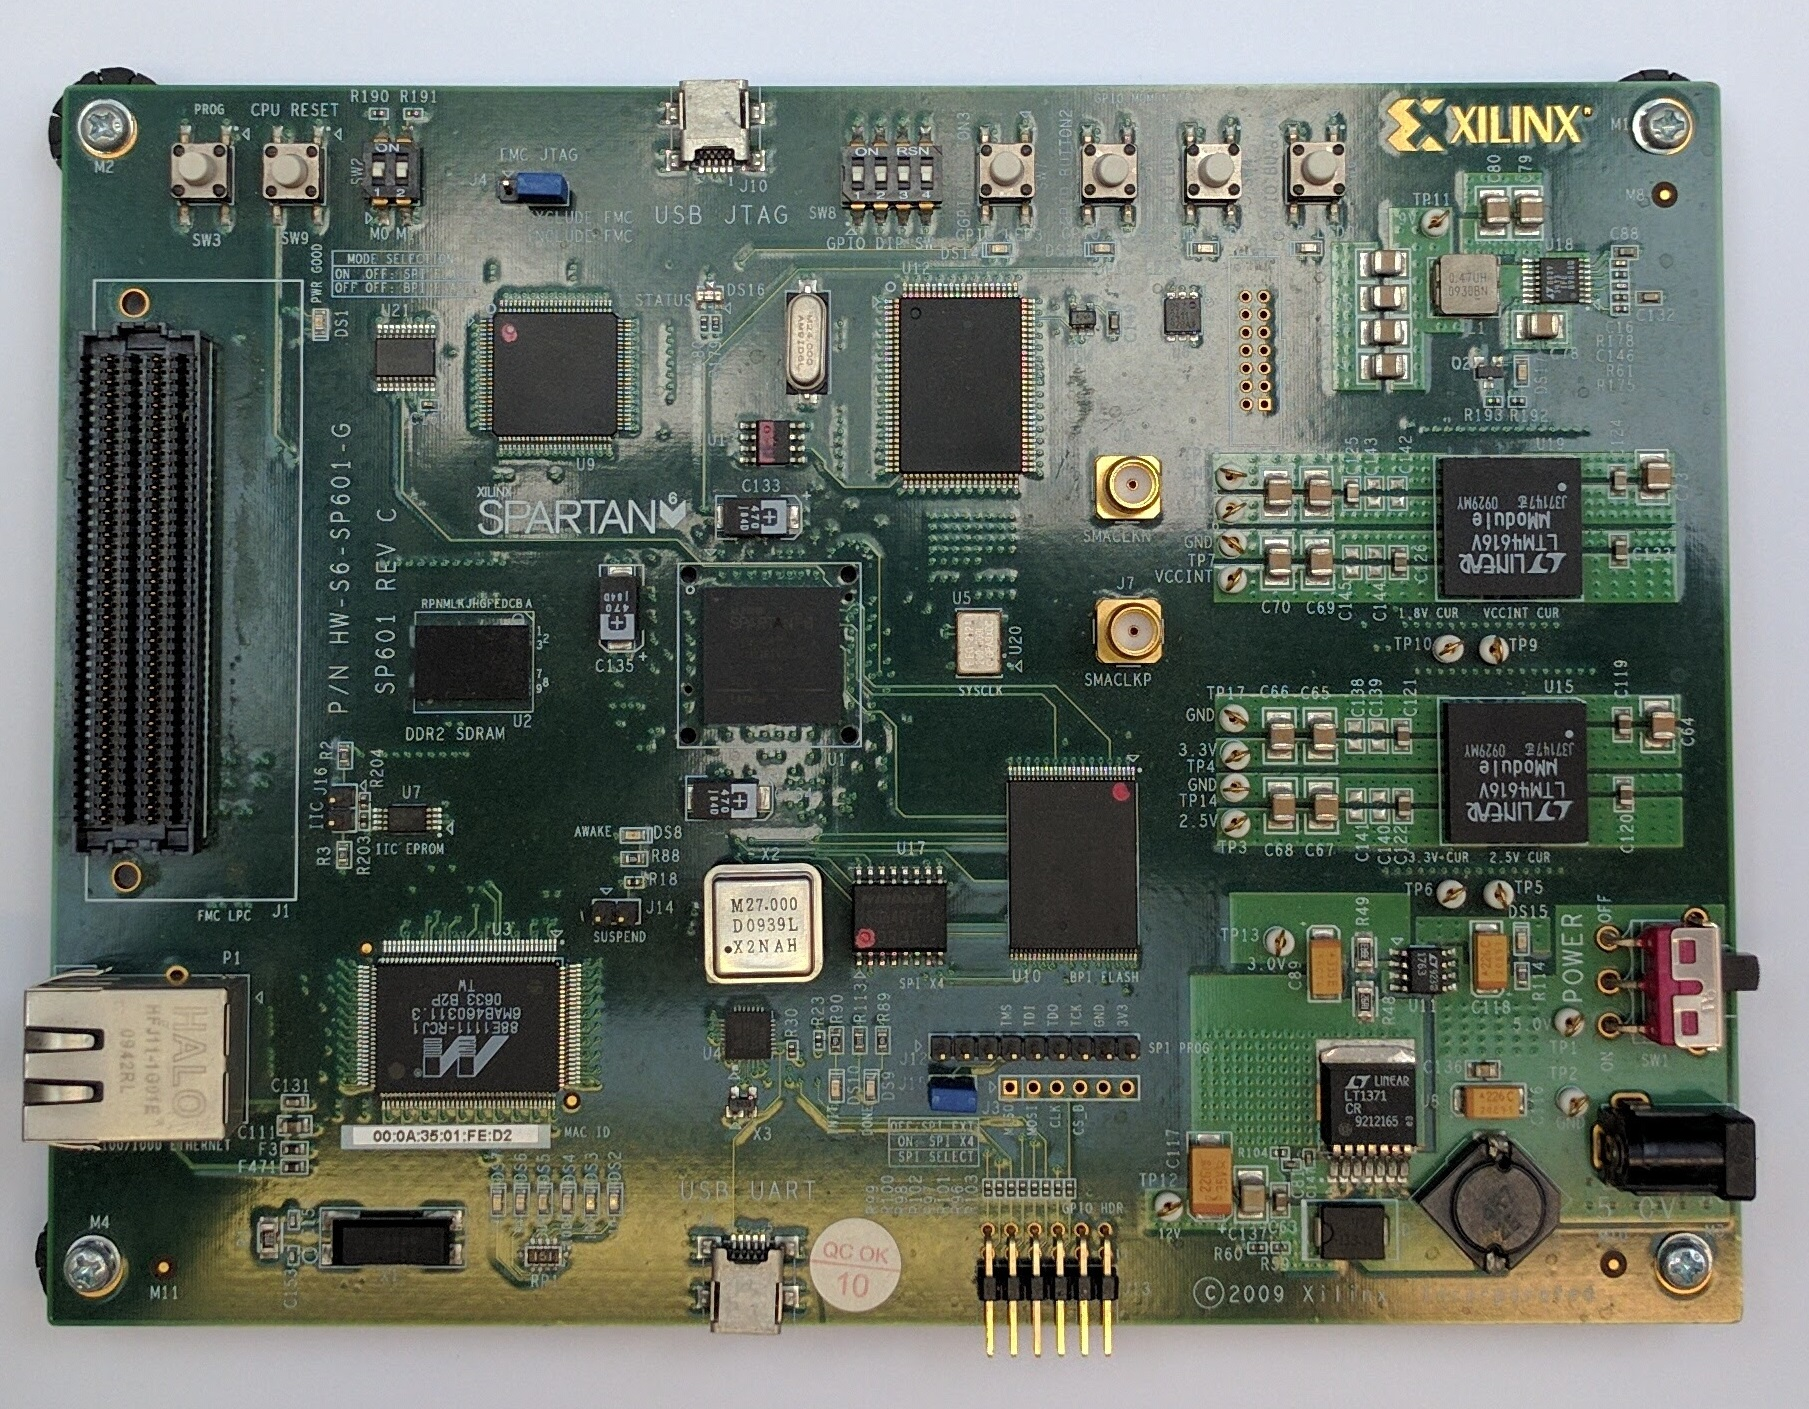
\includegraphics[width=0.7\textwidth]{img/III-2-web-daq/sp601.jpg}
      \caption{Photograph of the Xilinx SP601 development board showing the various components: the Spartan-6 FPGA in the middle, the SDRAM on its right, the Ethernet connector and MAC controller in the bottom-left corner, and the FMC connector on the left.}
      \label{fig:III-2-sp601}
    \end{figure}

    On the FPGA of the SP601, a dual-core Microblaze processor is implemented: one core handles the Ethernet connection and the other the communication with the VFAT2. The former runs a web server on top of the TCP/IP protocol in order to deliver the content of the web application used by the client to control and monitor the system ; the latter receives commands from the client and transfers them to the VFAT2. The whole system is contained in one board which can connect to various clients at the same time or to an external storage unit.

  \section{Web Server, WebSockets, and TCPSockets}

    A Microblaze processor is embedded on the FPGA of the SP601 and acts as web server to deliver web applications to clients which connect to the IP address of the board. Once the web application has been downloaded by the client over Hypertext Transfer Protocol (HTTP), real-time communication is established over WebSockets to transmit requests between parties. Figure \ref{fig:III-2-flow} displays the exchange of information between the client and the server.

    \begin{figure}[h!]
      \centering
      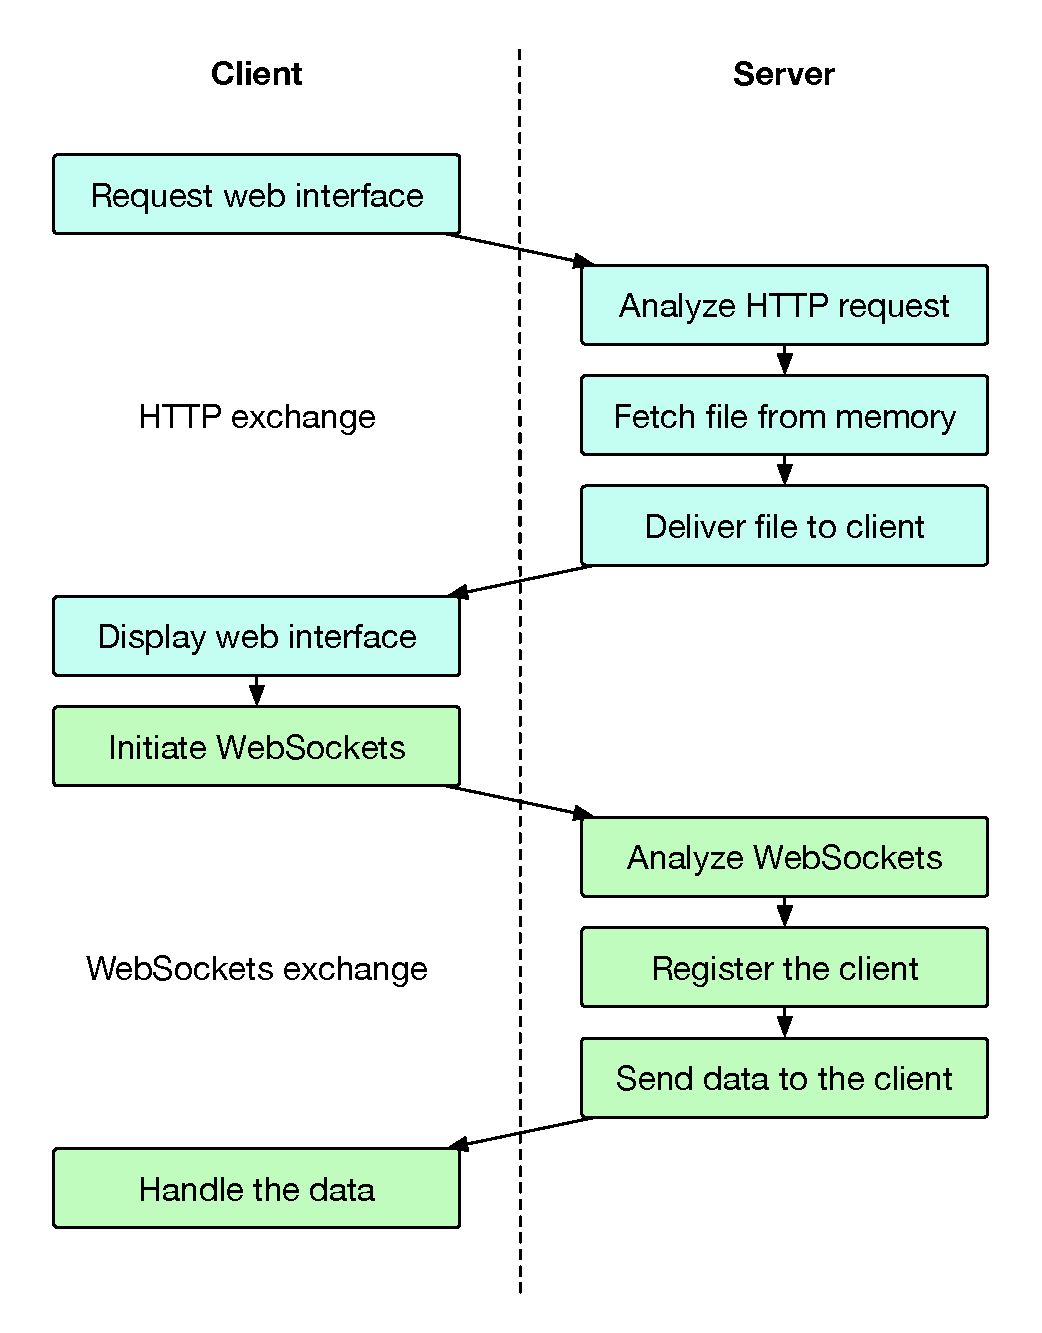
\includegraphics[width=0.8\textwidth]{img/III-2-web-daq/flow}
      \caption{Exchange of information between the client and the server.}
      \label{fig:III-2-flow}
    \end{figure}

    \subsection{The HTTP Standard}

      When an Internet browser pulls a web page from a server, it sends an HTTP request containing the type of request and the path of the page. The type of request defines what the action of the client is. It can be GET, PUT, DELETE, etc which will respectively ask for a specific page, transfer content, delete content, etc. The path on the other hand can be a reference to a file to download or to a script to handle the new data. The request is encoded in ASCII characters and is thus human-readable. Figure \ref{fig:III-2-http} displays an example of an HTTP request and response in which the client requests a specific page and the server returns the content of that page. \\

      \begin{figure}[h!]
        \begin{tabularx}{\textwidth}{C{1}C{1}}
          \textbf{HTTP request} & \textbf{HTTP response} \\
        { \footnotesize
\begin{alltt}
\textcolor{Red}{GET} \textcolor{MidnightBlue}{/index.html} \textcolor{Plum}{HTTP/1.1} \newline
\textcolor{BurntOrange}{Host:} www.web-daq.com
\end{alltt} } & { \footnotesize
\begin{alltt}
\textcolor{Plum}{HTTP/1.1} \textcolor{LimeGreen}{200 OK} \newline
\textcolor{BurntOrange}{Date:} Thu, 28 July 2016 10:36:02 GMT \newline
\textcolor{BurntOrange}{Content-Type:} text/plain; charset=UTF-8 \newline
\textcolor{BurntOrange}{Content-Encoding:} UTF-8 \newline
\textcolor{BurntOrange}{Content-Length:} 29 \newline
\textbf{This is the web application !}
\end{alltt} }
        \end{tabularx}
        \caption{Transcript of an HTTP request and response in which the client requests a specific page and the server returns the content of that page.}
        \label{fig:III-2-http}
      \end{figure}

      After analyzing the HTTP request, the server performs the desired operation and returns a status code, information headers, and optionally data. The status codes are defined in the HTTP standard: 200 means the operation was successful, 404 means that the request file is missing, 500 means the server encountered an error, etc. The additional headers contain information regarding the type of content that is returned (text, image, etc), the encoding of the data, the data size, etc. Finally, the response ends with the raw data. \\

      To each request, a single response is provided by the server. Moreover, the server does not initiate requests, meaning the communication has to be started by the client; the server can not push data to the client, but only provided data when probed (pulled).

    \subsection{The WebSockets Protocol}

      To allow the server to push data and enable real-time communication, the WebSockets standard was developed. WebSockets are sockets that can be used inside the Internet browser to communicate with a server following a given data format. When a connection is established, it remains open on both sides reducing the overhead on each data packet and decreasing the latency. \\

      Upon connection from a client to the server, a dedicated HTTP request is sent informing the latter that the WebSockets protocol is being used. Figure \ref{fig:III-2-websocket} shows the request and response that are sent during the handshaking procedure between the client and the server. The request contains an upgrade header which informs the server of the change of communication protocol, along with a random key. The response from the server informs the client that the switch was made and returns a hash which prevents multiple connections from a same client. The server stores the information of the client in a list of active users until the latter disconnects or the connection times out. After this handshaking procedure, data can be sent between parties without restriction.

      \begin{figure}[h!]
        \begin{tabularx}{\textwidth}{C{1}C{1}}
          \textbf{Handshake  request} & \textbf{Handshake response} \\
        { \footnotesize
\begin{alltt}
\textcolor{Red}{GET} \textcolor{MidnightBlue}{/websocket} \textcolor{Plum}{HTTP/1.1} \newline
\textcolor{BurntOrange}{Host:} www.web-daq.com \newline
\textcolor{BurntOrange}{Upgrade:} websocket \newline
\textcolor{BurntOrange}{Connection:} Upgrade \newline
\textcolor{BurntOrange}{Sec-WebSocket-Key:} x3JJHMbDL1EzLkh9GBhXDw== \newline
\textcolor{BurntOrange}{Sec-WebSocket-Protocol:} chat \newline
\textcolor{BurntOrange}{Sec-WebSocket-Version:} 13 \newline
\textcolor{BurntOrange}{Origin:} www.web-daq.com
\end{alltt} } & { \footnotesize
\begin{alltt}
\textcolor{Plum}{HTTP/1.1} \textcolor{LimeGreen}{101 Switching Protocols} \newline
\textcolor{BurntOrange}{Upgrade:} websocket \newline
\textcolor{BurntOrange}{Connection:} Upgrade \newline
\textcolor{BurntOrange}{Sec-WebSocket-Accept:} HSmrc0sMlYUkAGmm5OPpG2HaGWk= \newline
\textcolor{BurntOrange}{Sec-WebSocket-Protocol:} chat
\end{alltt} }
        \end{tabularx}
        \caption{Transcript of the request and response that are sent during the handshaking procedure of the WebSockets protocol between the client and the server.}
        \label{fig:III-2-websocket}
      \end{figure}

    \subsection{Handling Client Requests}

      The server on the Microblaze processor handles both HTTP and WebSocket requests, differentiating them using the HTTP header as selection criteria. It then forwards them to two dedicated functions according to the type of request. \\

      For HTTP requests, the headers are extracted along with the type and path. Only GET requests need to be handled in this application, corresponding to the download of resources: web page, image, etc. In case the requested path is valid, the file is retrieved from memory and sent back to the user. Otherwise, an error 404 is generated to inform the user that the resource is not available. In normal operation mode, the client connects once to the server over HTTP to download the application and then switches over to WebSocket communication. The switching is done through JavaScript code present in the application that is executed by the client. \\

      Once the application is downloaded, the connection with the server over WebSockets is established automatically. The server registers the client and real-time communication between parties can begin.

    \subsection{The TCPSockets Implementation}

      Although WebSockets provide an implementation of sockets in the web browser, they also define a format for the data being transmitted. This limits the field of application to the connection between a WebSockets client and server. A more generic approach uses the TCPSockets, a raw implementation of sockets in the web browser which is still in experimental phase. This technology enables the connection between any systems that support TCP sockets, including databases. A direct communication between the client and the database can thus be established in order to retrieve stored data, effectively bypassing the need for an intermediary server.

  \section{The Microblaze Processor}

    Upon startup of the Microblaze processor, the operating system is loaded into the SDRAM memory and executed. To implement the server and handle data, various components require initialization. Figure \ref{fig:III-2-Microblaze} shows the boot-up sequence of the system highlighting the configuration of the various subsystems. First, the caches are enabled allowing for an increased interaction speed between the processor and memory. Then, the interrupt controller is initialized and interrupts from the multiple modules are registered. One of them is the timer which triggers at given interval in order to execute control routines periodically. Finally, three complex modules are initialized: a Lightweight TCP/IP stack (lwIP) which handles the networking protocol, Memory File System (MFS) which creates a virtual file system, and Mailboxes which handle the communication between processors.

    \begin{figure}[p!]
\begin{alltt}
--------------------------------------------------
--                                              --
--            Microblaze Web Server             --
--                                              --
--    Developer:                                --
--    Thomas Lenzi - thomas.lenzi@ulb.ac.be     --
--------------------------------------------------
\textcolor{MidnightBlue}{Initializing the system...}
> Enabling the caches...                     [\textcolor{Green}{OK}]
> Initializing the interrupt controller...   [\textcolor{Green}{OK}]
> Initializing the timer...                  [\textcolor{Green}{OK}]
> Initializing MFS...                        [\textcolor{Green}{OK}]
\textcolor{MidnightBlue}{Setting up the network interface...}
> Board IP: 192.168.1.10
> Netmask : 255.255.255.0
> Gateway : 192.168.1.1
> Initializing lwIP...
> Adding network interface...                [\textcolor{Green}{OK}]
> Starting network interface...              [\textcolor{Green}{OK}]
\textcolor{MidnightBlue}{Setting up the TCP protocol...}
> Creating the TCP PCB...                    [\textcolor{Green}{OK}]
> Binding to port...                         [\textcolor{Green}{OK}]
> Starting the TCP server...                 [\textcolor{Green}{OK}]

>> Request: HTTP                             [\textcolor{Green}{200}]
>> Request: HTTP                             [\textcolor{Red}{404}]
>> Request: HTTP                             [\textcolor{Red}{500}]
>> Request: HTTP                             [\textcolor{Red}{Unknown}]

>> Request: WebSockets Handshake             [\textcolor{Green}{Hi}]
>> Request: WebSocket Data                   [\textcolor{Green}{Text}]
>> Request: WebSocket Data                   [\textcolor{Green}{Binary}]
>> Request: WebSocket Data                   [\textcolor{Red}{Unknown}]
>> Request: WebSocket Disconnect             [\textcolor{Green}{Bye}]
\end{alltt}
      \caption{Boot-up sequence of the operating system of the MicroBlaze highlighting the configuration of the various subsystems.}
      \label{fig:III-2-Microblaze}
    \end{figure}

    \subsection{Lightweight TCP/IP stack}

      lwIP is a light weighted implementation of the TCP/IP stack designed specifically for embedded systems with limited resources. The notion of stack is a reference to the Open Systems Interconnection (OSI) model which characterizes the communication functions of a system by subdividing it in layers, each performing a given task. The model contains seven layers: physical, data link, network, transport, session, presentation, and application. lwIP handles the data link, network, transport, and session layers, providing the user with an API to implement the presentation, and application layers.

      \paragraph{The physical layer} defines the electrical specifications of the communication medium and the way bits are encoded on the signal line. In this application, an Ethernet connection is used as interface between the SP601 development board and the network.

      \paragraph{The data layer} formats the raw data stream into packets and enables communication between two directly connected nodes on the network. It communicates directly with the hardware that composes the physical layer to transfer bits through a given network interface. It controls the latter and handles the flow of data. In the TCP/IP stack, the data layer is handled by the Media Access Control (MAC) and setup during the initialization of the network interface.

      \paragraph{The network layer} provides arbitration over a set of systems connected to a complex network where nodes are not directly connected to each other. It provides an address to each node in order for data to be transfered or routed. The prominent protocol used by networking systems is the Internet Protocol which provides a unique IP address to each node.

      \paragraph{The transport and session layers} are built on top of the network layer to add functions like error recovery, flow control, timeout, etc. A lightweight protocol implemented at this level is UDP which provides connectionless communication between nodes. They communicate by sending simple data packets without prior communication or acknowledgment system. This yields in a fast yet unreliable protocol. TCP on the other hand implements a full handshaking procedure which allows for features like congestion and flow control or data recovery. This however results in a heavyweight structure that can limit the range of target systems.

      \paragraph{The presentation layer} handles the encoding of the data which might vary between the transport and application layer. It is responsible for the encryption of the stream.

      \paragraph{The application layer} is the layer with which the software interact. In this application, the software handles either HTTP or WebSockets packets. \\

      Using lwIP, a TCP server is started on the Microblaze and is set up to listen to any incoming connection on port 80, the default port used by Internet browsers. Upon reception of data, lwIP transfers the packet from its internal functions (transport and session layers) to user functions (presentation and application layers) which handle the HTTP and WebSockets requests.

    \subsection{Memory File System}

      When the client requests the download of a file from the Microblaze, MFS is used to retrieve the content from the SDRAM. MFS allows the operating system to maintain a virtual file system in the dynamic memory. This is required as the SP601 development board is not equipped with storage memory to host a fully fledge file system. Part of the SDRAM is allocated to MFS which initializes it using a precompiled image loaded upon startup. The image contains a tree of directories and documents which can be directly accessed from the software. MFS provides a range of functions to manipulate these files as if they where stored on a hard-drive.

    \subsection{Mailboxes for Dual Processor Architecture}

      To enable communication between the two processors which run different software, a mailbox system is implemented. Mailboxes are buffers which can be filled by either processors and are used to transmit small amount of data. Whenever a buffer is filled, an interrupt is sent to the processor in order to perform a read operation. The mailboxes are used to send instructions from the processor running the server to the one communicating with the VFAT2 and transferring back the response. \\

      From the web application, the client can send requests to the server through WebSockets, which are transfered between processors and forwarded to the VFAT2. The returned data then follows the opposite path back to the client. Data can be broadcasted to multiple clients in order to update the information on each instance of the application at once.

  \section{Innovation of the Architecture}

    The architecture used in most systems such as the one described in Chapter \ref{chap:III-1-arch} is shown in Figure \ref{fig:III-2-system-old}. The whole system relies on the presence of the server which acts as the central node connecting the clients, the database, and the electronics. All transactions are required to transit through it, slowing down the performance of the whole infrastructure when scaling up. Furthermore, the client needs to constantly pull data from the server and the database to keep informed of the changes happing in the system or those submitted by other clients. \\

    \begin{figure}[h!]
      \centering
      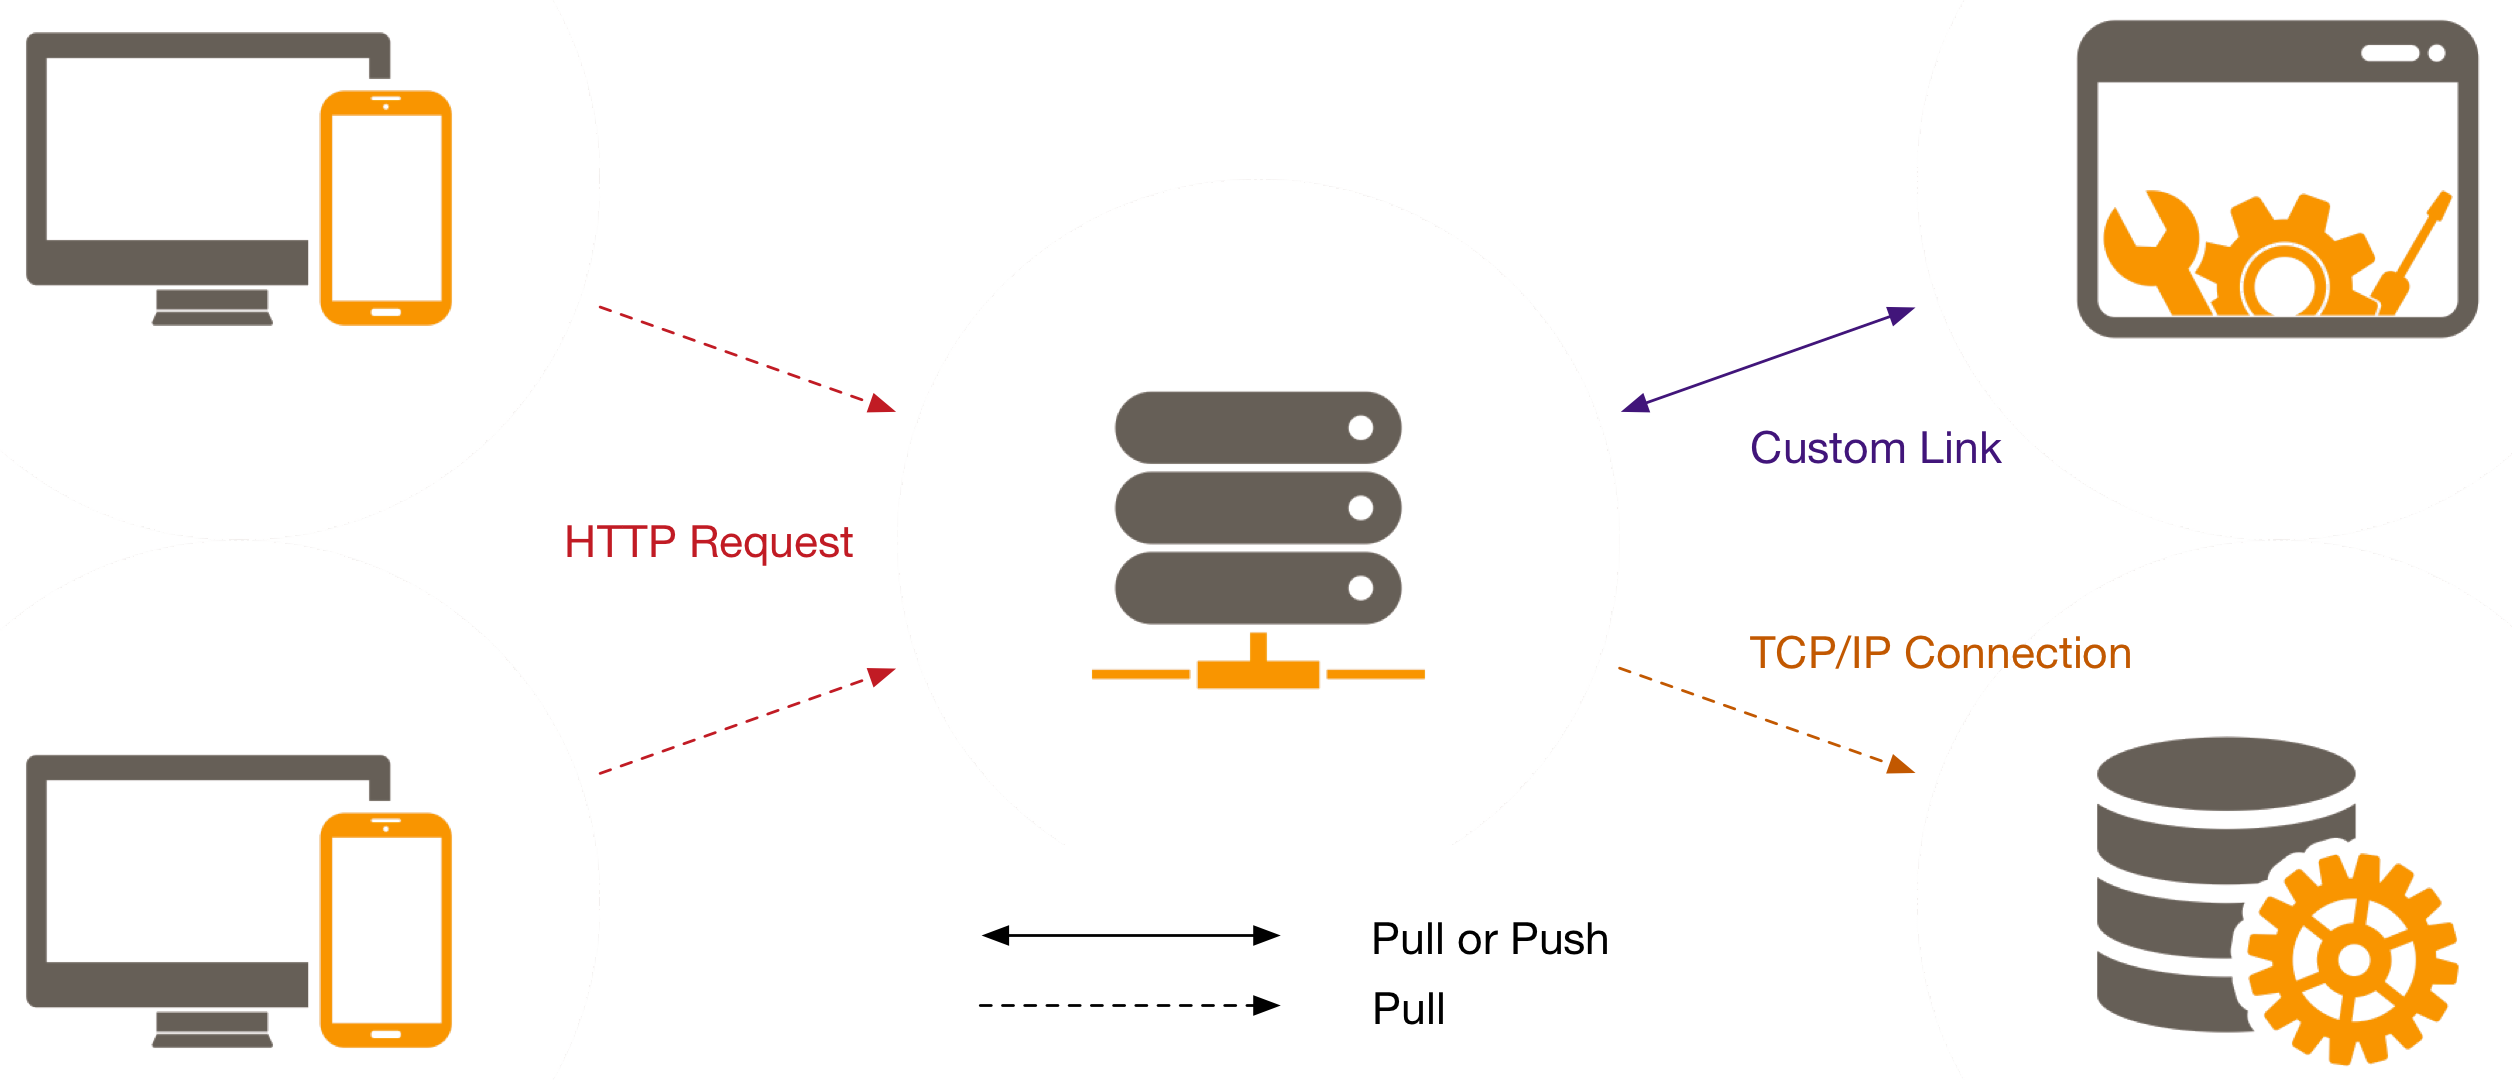
\includegraphics[width=0.8\textwidth]{img/III-2-web-daq/old-sys.png}
      \caption{Diagram of the architecture used in most DAQ systems in which the whole system relies on the presence of the server which acts as the central node.}
      \label{fig:III-2-system-old}
    \end{figure}

    The system described in this chapter moves away from a star network in which the server is the central piece and tries to form a mesh network where every component can directly access all other nodes. By taking advantage of the increase in computational power of microelectronics, it is possible to merge the functionalities of the server and the electronics in a single embedded system. Furthermore, developments in web technologies have enabled easy and reliable two-way communication between the client and the server and between the client and the database. The WebSockets technology provides response times up to ten times faster than classical solutions used to pull the server. The obtained system, which topology is shown in Figure \ref{fig:III-2-system-new}, thus allows for faster inter-node communication, which releases the traffic on given data paths, and allows for more bandwidth and activity. Furthermore, the distribution of the application is centralized by the server which transfer the most up-to-date version of the web pages to every client, ensuring compatibility across time and platforms. \\

    Through the two-way mesh network topology, each node can inform the systems of changes in real-time, effectively bypassing the need for a pull system which requests updated data at constant interval and generates unwanted traffic on the network. The system becomes truly real-time and event driven with minimum delays. The bandwidth allocated to each client on the network for a given number of client $ N $ goes from O(1/N) to O(1). As updates are pushed by the server, only one data packet is sent to all clients at once. Each client is not required to handle the pull system, each using up bandwidth.

    \begin{figure}[h!]
      \centering
      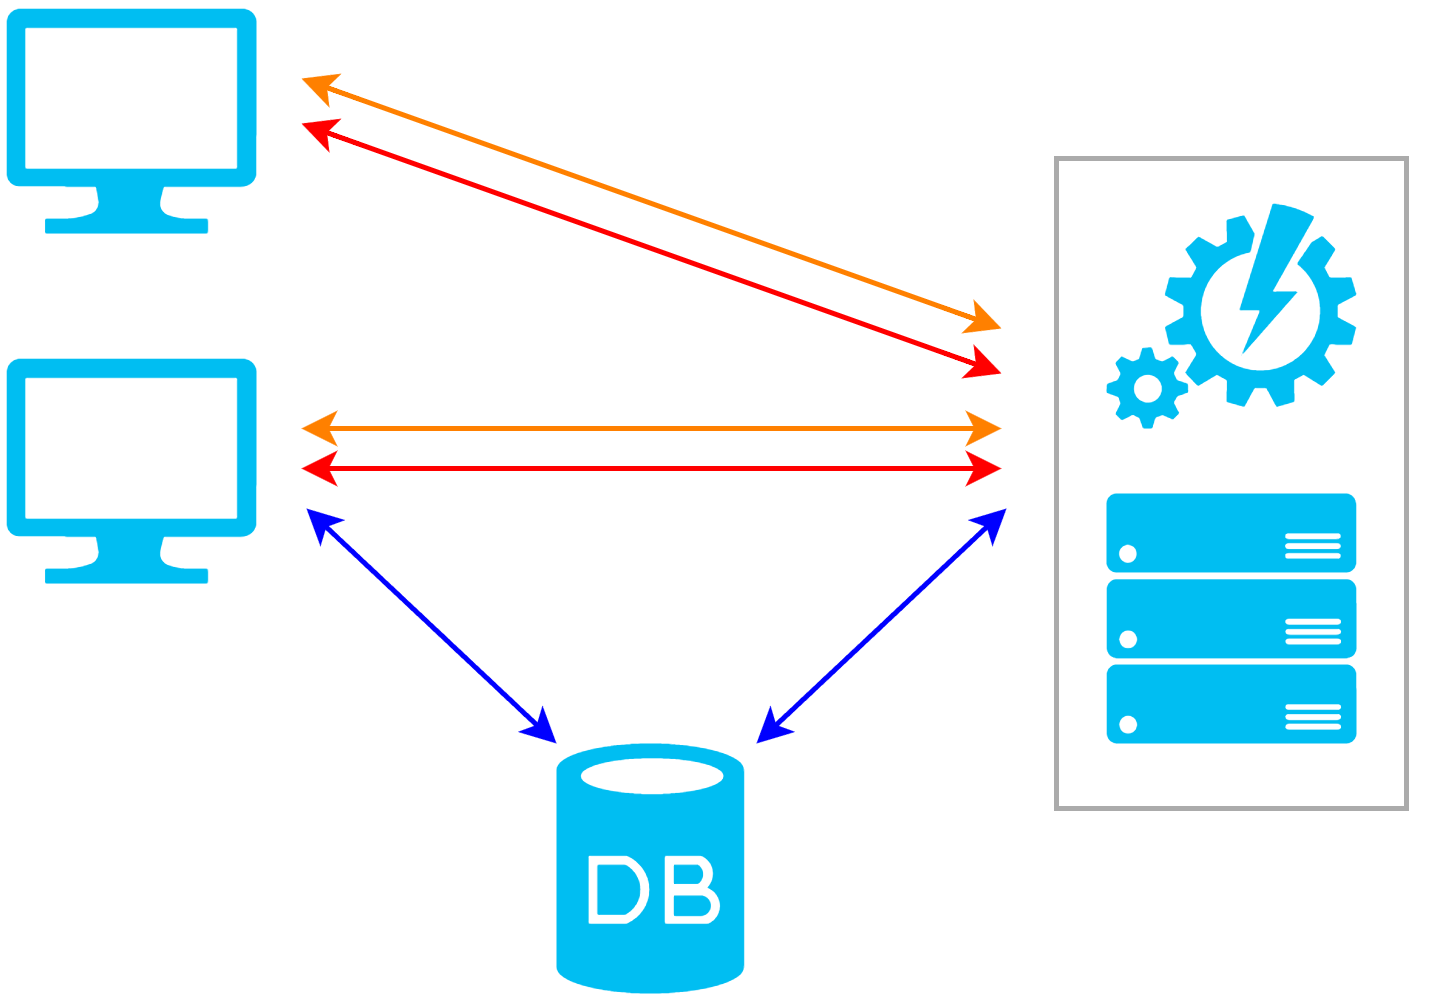
\includegraphics[width=0.8\textwidth]{img/III-2-web-daq/new-sys.png}
      \caption{Diagram of the new DAQ system which forms a mesh network where every component can directly access all other nodes.}
      \label{fig:III-2-system-new}
    \end{figure}

  \section{Conclusion}

    Using recent developments in web technologies, we were able to create an innovative data acquisition system architecture which provides higher flexibility and better utilizes the resources of the nodes in the network. Compared to classic designs which use pull/push techniques to transfer data, the new implementation offers event driven interactions, making use of the bandwidth only when necessary. \\

    Besides the increase in speed and optimization, the use of a web-based application offers greater portability on a variety of platforms without the need to maintain code for various systems. \\

    This system is a proof-of-concept for a new type of data acquisition systems which relies on event based data analysis and control. It has the advantage to offer great flexibility and reduce the complexity of the overall system, while deeply combining the electronics readout and the server providing data.
